\renewcommand{\LangOO}{\ensuremath{{\mathcal{L}}_{ul}}\xspace }

\section{The underlying programming language \LangOO}  
\label{sect:underlying}

\subsection{\LangOO syntax and runtime configurations}
\label{sub:Loo} 
This work is based on \LangOO, a {minimal}, imperative, sequential,  class based, typed, object-oriented language. 
We believe, however, that the work can easily be adapted to any capability safe language with some form of encapsulation. 
Wrt to encapsulation and  capability safety,  \LangOO supports private fields, private and public methods, unforgeable addresses, and no ambient authority (no static methods, no address manipulation).
To reduce the complexity of our formal models, as is usually done, CITE - CITE,  \LangOO lacks many
common languages features, omitting static fields and methods, interfaces,
inheritance, subsumption, exceptions, and control flow.  
  It has a simple concept of module with module-private fields and methods, described in Sect. \ref{sect:execution}.
 
 
 The syntax of \LangOO is given in Fig. \ref{f:loo-syntax}. It  includes syntax for ghost terms $gt$ that may %only
be used in writing
specifications or the definition of ghost fields.
 The operational semantics of \LangOO~ {is given  in   {Appendix \ref{app:loo}.}\footnote{{{The examples in this paper are using  a slightly richer syntax for greater readability.}}}
 A \LangOO state, $\sigma$,  consists of a  heap $\chi$ and a stack. 
{A stack  is a sequence of frames, $\phi_1\!\cdot\!...\!\cdot\! \phi_n$.}
A  frame, $\phi$, consists of a local variable map and a continuation, \ie a sequence of statements to be executed.
The top frame, \ie  the frame most recently pushed onto the stack,  in a state $(\phi_1\!\cdot\!...\!\cdot\! \phi_n, \chi)$ is $\phi_n$.



\begin{figure}[t]
\footnotesize{
$
 \begin{array}{ll}
 \begin{syntax}
\syntaxElement{Mdl}{Module Def.}
		{
		\syntaxline{\overline{C\ \mapsto\ CDef}}\endsyntaxline
		}
\endSyntaxElement\\
\syntaxElement{CDef}{Class Def.}
		{
		% [An]\
		 \prg{class}\ C\ 
		\{\  \overline{fld}; \overline{mth};\  \overline{gfld};\  \}		
		}
\endSyntaxElement 
\\
\syntaxElement{mth}{Method Def.}
		{
		\syntaxline
		{ {p}\  \prg{method}\ m\ (\overline{x : T}){:T}\{\ s\ \} }
		\endsyntaxline
		}
\endSyntaxElement
\end{syntax}
 &    
\begin{syntax}
\syntaxElement{fld}{Field Def.}
		{\syntaxline
			{\prg{field}\ f\ :\ T}
		\endsyntaxline}
\endSyntaxElement 
\\
\syntaxElement{T}{Type}
		{
		\syntaxline
				{C}
		\endsyntaxline
		}
\endSyntaxElement
\\
\syntaxElement{p}{Privacy}
		{
		\syntaxline
		{\prg{private}}
		{\prg{public}}
		\endsyntaxline
		}
\endSyntaxElement 
\end{syntax}

 \end{array}
 $
\\
\[
\begin{syntax}
%\syntaxElement{Mdl}{Module Def.}
%		{
%		\syntaxline{\overline{C\ \mapsto\ CDef}}\endsyntaxline
%		}
%\endSyntaxElement\\
%\syntaxElement{CDef}{Class Def.}
%		{
%		% [An]\
%		 \prg{class}\ C\ 
%		\{\  \overline{fld}; \overline{mth};\  \overline{gfld};\  \}		
%		}
%\endSyntaxElement\\
%%\syntaxElement{An}{Class Annotation}
%%		{\enclosed}
%%\endSyntaxElement\\
%\syntaxElement{fld}{Field Def.}
%		{\syntaxline
%			{\prg{field}\ f\ :\ T}
%		\endsyntaxline}
%\endSyntaxElement 
%\\
%\syntaxElement{T}{Type}
%		{
%		\syntaxline
%				{C}
%		\endsyntaxline
%		}
%\endSyntaxElement
%\\
%\syntaxElement{mth}{Method Def.}
%		{
%		\syntaxline
%		{ {p}\  \prg{method}\ m\ (\overline{x : T}){:T}\{\ s\ \} }
%		\endsyntaxline
%		}
%\endSyntaxElement\\
%\syntaxElement{p}{Privacy}
%		{
%		\syntaxline
%		{\prg{private}}
%		{\prg{public}}
%		\endsyntaxline
%		}
%\endSyntaxElement 
%\\
\syntaxElement{s}{Statement}
		{
				\syntaxline
				{{x:=y}}
				{{x:=v}}
				{x:=y.f}
				{x.f:=y}
				{x:=y_0.m(\overline{y})}
				{\prg{new} \ {C} }
				{ s;\ s }
				  { \epsilon }
			       \endsyntaxline
		}
\endSyntaxElement
\\
%\syntaxElement{c}{Continuation}
%		{
%		\syntaxline
%				{{s; \ x}}
%				{{x}}
%		\endsyntaxline
%		}
%\endSyntaxElement\\
\syntaxElement{gfld}{Ghost Field Def.}
		{\syntaxline
			{\prg{ghost}\ g\ (\overline{x : T})\{\ gt\ \} : T}
%			{\prg{ghost}\ \prg{intrnl}\ g\  (\overline{x : T})\{\ gt\ \} : T}
		\endsyntaxline}
\endSyntaxElement\\
\syntaxElement{{gt}}{{Ghost Term}}
		{
		\syntaxline
				{x}
				{v}
				{gt\! +\! gt}
				{gt\! =\! gt}
				{gt \!< \!gt}
				{gt.f}
				{gt.g(\overline {gt})}
		\endsyntaxline
		}
		{
		\syntaxline
		{\prg{if}\ gt\ \prg{then}\ gt\ \prg{else}\ gt}
		\endsyntaxline
		}
\endSyntaxElement
\\
\end{syntax}
\]
\\
 $
 \begin{array}{lcl}
 \begin{syntax}
\syntaxElement{\sigma}{Program {State}}
		{
		\syntaxline
		{( \overline \phi, \chi )}
		\endsyntaxline
		}
\endSyntaxElement 
\\
% SD Stack is implictt now
%\syntaxElement{\psi}{Stack}
%		{\syntaxline{\phi}{\phi {\cdot} \psi}\endsyntaxline}
%\endSyntaxElement\\
\syntaxElement{\phi}{Frame}
		{
		\syntaxline
		{  (\  \overline{x\mapsto v};\ s \ ) }
		\endsyntaxline
		}
\endSyntaxElement\\
\syntaxElement{\chi}{Heap}
		{(\  \overline{\alpha \mapsto o}\ )}
\endSyntaxElement
\end{syntax}
 & \hspace{1cm} & 
\begin{syntax}
\syntaxElement{o}{Object}
		{(\ C;\  \overline{f \mapsto v} \ )}
\endSyntaxElement\\
\syntaxElement{v}{Value}
		{
		\syntaxline
				{\alpha}
				{i}
				{\true}
				{\false}
				{\nul}
		\endsyntaxline
		}
\endSyntaxElement
\end{syntax}

 \end{array}
 $
 }
\caption{\LangOO Syntax. We use $x$, $y$, $z$ for variables, \ $C$, $D$ for class identifiers, $f$ for field identifier, $g$ for ghost filed identifiers, $m$ for method identifiers, $\alpha$ for addresses, $i$ for integers.
}
\label{f:loo-syntax}
\end{figure}


 
 
\paragraph{Notation} We adopt the following unsurprising notation:
\label{s:notation}
\begin{itemize}
\item
{An object is uniquely identified by the address that points to it. We shall be talking of objects $o$, $o'$ when talking less formally, and of addresses, $\alpha$, $\alpha'$, $\alpha_1$, ...  when more formal.}
\item
$x$, $x'$, $y$, $z$, $u$, $v$, $\va$  are {variables}. 
\item
$dom(\phi)$ and $Rng(\phi)$ indicate the variable map in $\phi$; \ \ $dom(\sigma)$ and $Rng(\sigma)$ indicate the variable map in the top frame in $\sigma$
\item
$\alpha \in \sigma$ means that $\alpha$ is defined in the heap of $\sigma$, and $x\in \sigma$ means that $x\in dom(\sigma)$.
Conversely,  $\alpha\notin\sigma$ and $x\notin\sigma$ %, and $\va \notin A$ h
 have the obvious meanings.
$\interpret{\sigma}{\alpha}$  is $\alpha$; and $\interpret{\sigma}{x}$  is the value to which  $x$  is mapped in the top-most frame of $\sigma$'s stack, 
and $\interpret{\sigma}{e.f}$ looks up in $\sigma$'s heap the value of $f$ for the object  $\interpret{\sigma}{e}$.
% too much detail?
% Note that $\interpret{\sigma}{e}$ is not defined when $e$ contains a method call or a ghost field.
\item %The  update
$\phi[x \mapsto \alpha]$ updates  the variable map  of $\phi$,  
and  $\sigma[x \mapsto \alpha]$ updates the top frame of $\sigma$.
\item
$A[e/x]$ is textual substitution where we replace all occurrences of $x$ in $A$ by $e.$ 
\item
As usual, $\overline q$ stands for  sequence $q_1$, ... $q_n$, where $q$ can be an address, a variable,    a frame, an update or a substitution.
Thus,   $\sigma[\overline{x \mapsto \alpha}]$ and $A[ \overline{e/y}]$ 
% applies the substitutions $\overline{x \mapsto \alpha}$ to the top frame.
have the expected meaning.
\item
$\phi.\prg{cont}$ is the continuation of frame $\phi$, and  $\sigma.\prg{cont}$ is the continuation in the top frame.
\item
$text_1 \txteq text_2$ expresses that $text_1$ and $text_2$ are  the same text.%textually equal.
% the below moved to appendix
%  $s_1 \txtin   s_2$  means  $s_1 \txteq  s_2$ or  $s_2 \txteq  s_1; s_3$ for some $s_3$, where $s_1$, $s_2$, and $s_3$ are program statements. 
\item
We define the depth of a stack as $\DepthFs {\phi_1...\phi_n} \triangleq n$. For states, $\DepthSt {(\overline \phi, \chi)} \triangleq  \DepthFs {\overline \phi}$.
The  operator $\RestictTo  \sigma k$ truncates the stack up to the $k$-th frame: % from $\sigma$. Namely, 
 $\RestictTo {(\phi_1...\phi_k...\phi_n,\chi)} {k}  \triangleq   (\phi_1...\phi_k,\chi)$
\item
{ $\vs(stmt)$ returns the variables which appear in $stmt$. For example, $\vs(u:=y.f)$=$\{u,y\}$.}
\end{itemize}

  

  
\subsection{\LangOO Execution}
\label{sect:execution}

 \LangOO execution is described by a small steps operational semantics of the shape $\leadstoOrig  {\Mtwo} {\sigma}   {\sigma'}$ 
 -- {\cf Fig. \ref{f:evaluation}.} 
  $\Mtwo$ stands for one or more modules, where a
  module,  $M$, maps class names to class definitions. 
{The semantics enforces dynamically a simple form of module-wide privacy: 
Fields may be read or written only if the class of the object whose field is being read or written, and the class of the object which is reading or writing belong to the same module.}
Private methods may be called only if the class of the receiver (the object whose method is being called), and the class of the caller (the object which is calling) belong to the same module.
Public methods may always be called.

The semantics is unsurprising :  
In $\sigma$, the  top frame's continuation contains the statement to be  executed next.  
 Statements may assign to variables, allocate new objects, 
perform field reads and writes on objects, and
 call methods on those objects. 
When a method is called, a new frame is pushed onto the stack; this frame  maps \prg{this} and the formal parameters to  the values for the receiver and other arguments, and the continuation to the body of the method. 
{Methods are expected to store their return values in the variable \prg{res}.}
 When the continuation is {empty ($\epsilon$), the frame is popped and the value of \prg{res}
 {\susan{\footnote{\prg{res} is implicit like \prg{this}}}}
 {\footnote {\sue{In the examples in this paper \prg{void} methods omit the assignment to \prg{res}.}}}
 from the popped frame  is stored  in the variable map of the top frame.}
%In other aspects, the semantics is unsurprisring.%we return from that call, its frame is  popped, and execution continues in the context of the calling method. 
%The relation $\leadstoOrigStar  {\Mtwo} {\_}   {\_}$  is the reflexive, transitive closure of $\leadstoOrig  {\Mtwo} {\_}   {\_}$ .
Wlog, {to simplify some proofs} we  require, as in Kotlin, that method bodies do not assign to formal parameters, , \cf Def.  \ref{def:wf:state}.  
%This simplifies some proofs and gives rise to a well-formedness requirement for states, 
%$\models \sigma$, which guarantees that for all frames  on the stack, the actual parameters of a method call in a  caller frame have the same values as the formal parameters in the called frame, \cf Def.  \ref{def:wf:state}. 
%From now on we require implicitly that $\models \sigma$.

Fig. \ref{fig:illusrPreserve}  from \S \ref{s:outline} % \ref{fig:UpSemantics}
 illustrates  such  ${\leadstoN}$ executions. We distinguish
  steps within the same  call ($\rightarrow$),\   entering a method  ($\uparrow$),\    returning from a method  ($\downarrow$).
Thus,  $\sigma_8 \rightarrow \sigma_9$ indicates that  $\leadstoOrig {\Mtwo}{\sigma_8}   {\sigma_9} $ is a step within the same call, 
\ $\sigma_9 \uparrow \sigma_{10}$ indicates that $\leadstoOrig {\Mtwo}{\sigma_9}   {\sigma_{10}} $ is a method entry, \ with 
  $\sigma_{12} \downarrow \sigma_{13}$   the corresponding return. 
In general,  $\leadstoOrigStar  {\Mtwo} {\sigma}   {\sigma'}$ may involve  any number of  calls or returns: \eg
 $\leadstoOrigStar  {\Mtwo} {\sigma_8}   {\sigma_{12}}$ involves one call and no return,
while $\leadstoOrigStar  {\Mtwo} {\sigma_{10}}   {\sigma_{15}}$,   involves no calls and two returns.


%\begin{figure}[htb]
%\begin{tabular}{|c|}
% \hline %  \\ -- this added one vertical space
%\resizebox{7cm}{!}{
%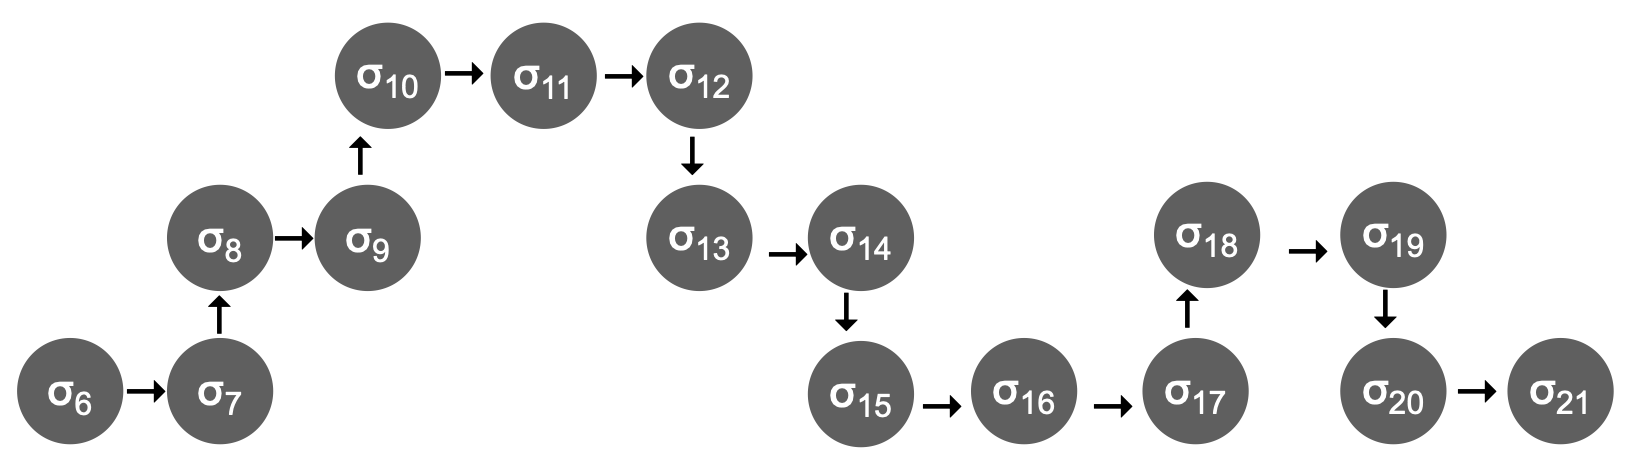
\includegraphics[width=\linewidth]{diagrams/bounded2.png}
%} 
% \\
%\hline
%
%\end{tabular}
%   \caption{$\rightarrow$:\  step within the same method; \ \ $\uparrow$:\    entering a method;\ \  $\downarrow$:  returning from a method}
%   \label{fig:UpSemantics}
% \end{figure}
 

\section{\susan{Fundamental} Concepts}
\label{s:auxiliary}

{The semantics of our assertion language % , \AssertLang, 
is based on three concepts built on} \LangOO: {method calls and returns, scoped execution}, and locally reachable objects.}

% \subsection{ Method Calls and Returns}
 
Method calls and returns are \susan{critical} for our work. 
They are characterized through pushing/popping   frames on the stack.  
The operator   $ \PushS  {\phi} {\sigma}$ pushes 
frame $\phi$ onto the stack of $\sigma$,
 \susan{ while
 operator $\sigma$ $\popSymbol$   pops a frame of $\sigma$'s stack and updates the continuation and variable map.}

 
 
\forget{
\begin{definition}
\label{def:push:frame}
Given a state $\sigma$, addresses $\overline \alpha$, a frame $\phi$,  variables or addresses $\overline \va$, we define
\begin{itemize}
\item
 $ \PushSF  {\phi} {\sigma} \ \triangleq \ ({\overline{\phi}\cdot\phi}, \chi)$ \ \ \  if \ \ \  $\sigma=(\overline{\phi}, \chi)$.
\item
$ \ \sigma\, \popSymbol \ \ \  \triangleq\   { (\overline{\phi}\cdot (\phi_n[\prg{cont}\mapsto stmt][x \mapsto \interpret {\phi_n}{ret}]), \chi)}$ \ \ \  if \\
 $\strut \hspace{1.2cm}  \exists x, y_0, \overline y. [ \ \sigma=(\overline{\phi}\cdot\phi_n\cdot\phi_{n+1}, \chi)$, and $\phi_n(\prg{cont})\txteq x:= y_0.m(\overline y); stmt \ ]$
\end{itemize}
 \end{definition}}
\begin{definition}
\label{def:push:frame}
Given a state $\sigma$, and a frame $\phi$,  we define
\begin{itemize}
\item
 $ \PushSF  {\phi} {\sigma} \ \triangleq \ ({\overline{\phi}\cdot\phi}, \chi)$ \ \ \  if \ \ \  $\sigma=(\overline{\phi}, \chi)$.
\item
$ \ \sigma\, \popSymbol \ \ \  \triangleq\   { (\overline{\phi}\cdot (\phi_n[\prg{cont}\mapsto stmt][x \mapsto \interpret {\phi_n}{\prg{res}}]), \chi)}$ \ \ \  if \\
 $\strut \hspace{1.5cm} \sigma=(\overline{\phi}\cdot\phi_n\cdot\phi_{n+1}, \chi)$, and $\phi_n(\prg{cont})\txteq x:= y_0.m(\overline y); stmt $
\end{itemize}
 \end{definition}

Consider Fig. \ref{fig:illusrPreserve}  again: $\sigma_8 = \PushSF  {\phi} {\sigma_7}$ for some $\phi$, and  $\sigma_{15}$=$\sigma_{14} \popSymbol$
--  thus $\sigma_8$ is a {\emph{called}} state for 
 $\sigma_7$, and  $\sigma_{15}$ is the {\emph{return}} state from 
 $\sigma_{14}$.
% Note that $\sigma = \sigma' \popSymbol$ iff $\sigma'\!\in\!\PushS  {\phi} {\sigma}$; we can see that 
% Also, 
% $\sigma_{14}\!\in\!\PushS  {\phi'} {\sigma_{15}}$ for some $\overline {\alpha'}$ -- {thus $\sigma_{15}$ is a caller state for  $\sigma_{14}$}.
%\footnote{$\phi'$ may differ from $\phi$, because between $\sigma_8$ and $\sigma_{15}$ there may 
% have been assignments to local variables.} 

 
 \subsection{Scoped Execution}
 \label{sect:bounded}


In order to give semantics to scoped invariants (introduced in \S  \ref{sect:approach:scoped} and to be fully defined  in Def.  \ref{def:necessity-semantics}), we need a new definition of execution, called \emph{scoped execution}. 

 
 \renewcommand{\EarlierS}[2]{\DepthSt{#1} \leq \DepthSt{#2}}
 \renewcommand{\NotEarlierS}[2]{\DepthSt{#1} \not\leq \DepthSt{#2}} 
 
\begin{definition}[Scoped Execution]:
\label{def:shallow:term}
 
\begin{itemize}

  \item
{  $\leadstoBounded  {\Mtwo} {\sigma}   {\sigma'} \ \ \   \,   \ \ \ \triangleq \ \ \  \leadstoOrig {\Mtwo} {\sigma} {\sigma'} \, \wedge\, 
 \EarlierS {\sigma}  {\sigma'} $}
  \item
{  $\leadstoBoundedStar {\Mtwo}  {\sigma_1}  {\sigma_n}  \ \ \,  \ \    \ \triangleq  \ \ \  {\sigma_1} = {\sigma_n}\ \ \vee \ \  \exists \sigma_2,...\sigma_{n-1}.\forall i\!\in\! [1..n)[\  \leadstoOrig {\Mtwo}  {\sigma_i}  {\sigma_{i+1}}\  \wedge\  \EarlierS{\sigma_1} {\sigma_{i+1}} \ ]$ }
% \wedge\,  \EarlierS{\sigma_1} {\sigma_n}$}\ \  
\item
  $\leadstoBoundedStarFin {\Mtwo}  {\sigma}  {\sigma'}  \  \,  \ \  \ \triangleq  \ \ \  \leadstoBoundedStar {\Mtwo}  {\sigma}  {\sigma'}  \ \wedge\ \
 {\DepthFs \sigma = \DepthFs {\sigma'} \ \ \wedge \ \ \sigma'.\prg{cont}=\epsilon  } $
 \end{itemize}
\end{definition}


Consider    Fig. \ref{fig:illusrPreserve} :
Here $\EarlierS {\sigma_8} {\sigma_9}$ and thus $\leadstoBounded   {\Mtwo} {\sigma_8} {\sigma_9}$. Also,  {$\leadstoOrig {\Mtwo} {\sigma_{14}}  {\sigma_{15}}$  but  $\NotEarlierS {\sigma_{14}} {\sigma_{15}} $  (this step returns from the active call in $\sigma_{14}$), and hence   $\notLeadstoBounded  {\Mtwo}  {\sigma_{14}}   {\sigma_{15}}$. 
Finally, even though $\DepthSt {\sigma_8} = \DepthSt {\sigma_{18}}$
%$\sigma_8$ and $\sigma_{18}$ have the same depth of stack 
 and $\leadstoOrigStar {\Mtwo} {\sigma_8}  {\sigma_{18}}$, we have  
 $\notLeadstoBoundedStar {\Mtwo} {\sigma_8}   {\sigma_{18}}$: in 
This is so, because the execution $\leadstoOrigStar {\Mtwo} {\sigma_8}  {\sigma_{18}}$ goes through the step
$\leadstoOrig {\Mtwo} {\sigma_{14}}  {\sigma_{15}}$ and  $\NotEarlierS {\sigma_{8}} {\sigma_{15}} $
 (this step returns from the active call in  $\sigma_8$).

\vspace{.1cm}
{The relation $\boundedTrans$ contains more than the transitive closure of  $\bounded$.
\Eg, ${\leadstoBoundedStar  {\Mtwo}  {\sigma_9}  {\sigma_{13}}}$, even though ${\notLeadstoBounded   {\Mtwo}  {\sigma_{12}}  {\sigma_{13}}}$.} 
%
Appendix \ref{app:aux} discussed further properties of scoped execution:
%Lemma \ref{lemma:orig:to:bounded:front} says  that \scoped executions describe the same set of executions as those  starting at an initial state\footnote{An \emph{Initial} state's heap contains a single object of class \prg{Object}, and
%its  stack   consists of a single frame, whose local variable map is a mapping from \prg{this} to the single object, and whose continuation is  any statement.
%(See Def. \ref{def:initial})}. 
%{Lemma \ref{l:var:unaffect} says that scoped execution does not affect the contents of variables in earlier frames.}
%and that 
%the interpretation of a variable remains unaffected by
%scoped execution of statements  which do not mention that variable.

 








  \subsection{Reachable  Objects, and Locally Reachable Objects}
  
 {A central concept to our work is %object 
protection, \se{that no locally reachable external object can have %unmitigated
\se{direct} access to that object}. We define it formally in  Sect. \ref{sect:protect}}
An object
% $\alpha'$ is  \emph{reachable} from another object $\alpha$, i.e., $\alpha' \in  \Relevant \alpha   \sigma $, if there is path from $\alpha$ to $\alpha'$; and 
$\alpha$ is
 \emph{locally reachable}, i.e. $\alpha \in  \LRelevantO   \sigma $, if it is reachable from the top frame on the stack of $\sigma$.
 
\begin{definition} We define 
\begin{itemize}
\item
{{$\Relevant {\alpha} {\sigma}  \ \ \ \ \ \triangleq \ \  \  \{ \ \alpha' \, \mid \ \exists n\!\in\!\mathbb{N}.\exists f_1,...f_n.. [\ \interpret {\sigma} {\alpha.f_1...f_n} = \alpha'\ \}$}}.
\item
$ \LRelevantO   \sigma  \ \  \ \triangleq \ \  \  \{ \ \alpha \ \mid \ { \exists x\in dom(\sigma) \wedge \alpha \in \Relevant {\interpret  {\sigma} x}
{\sigma} \ \} } $.
% \exists n\!\in\!\mathbb{N}.\exists f_1,...f_n, x. [\ \interpret {\sigma} {x.f_1...f_n} = \alpha\ ]$}
\end{itemize}
\end{definition}

 
Lemma  \ref{lemma:relevant} % describes properties of global reachability. 
says that 
(\ref{oneLR}) any object which is locally reachable after pushing a frame was locally reachable before pushing that frame, and 
(\ref{threeLR}) a pre-existing object, locally reachable after any number of scoped execution steps, was locally reachable at the first step.
\footnoteSD{cite ``only connectivity begets connectivity''}

\begin{lemma}
\label{lemma:relevant}
\label{lemma:push:N}
For all modules $\Mtwo$, states $\sigma$, $\sigma'$,   and frame $\phi$:
\begin{enumerate}
\item
\label{oneLR}
{$ \sigma'= \PushS {\phi} {\sigma}   \ \wedge  \  {Rng(\phi)} \subseteq \LRelevantO  {\sigma} 
 \ \  \Longrightarrow\ \ \LRelevantO {\sigma'}\  \subseteq \LRelevantO   {\sigma}$}
\item
\label{threeLR}
{${\leadstoBoundedStar {\Mtwo}  {\sigma}    {\sigma'}}  \ \  \Longrightarrow\ \ 
dom(\sigma) \cap \LRelevantO {\sigma'} \subseteq   \LRelevantO {\sigma}$
}

\end{enumerate}
\end{lemma}

{Consider Fig.  \ref{fig:illusrPreserve} . %, and Fig.  \ref{fig:UpSemanticsBounded}.
Lemma \ref{lemma:relevant}, part \ref{threeLR}  promises that any objects locally reachable in $\sigma_{14}$ which already existed in $\sigma_{8}$, were locally reachable in $\sigma_{8}$. However, the lemma is only  applicable to scoped execution, and as 
$\notLeadstoBoundedStar {\Mtwo} {\sigma_8}  {\sigma_{17}}$, 
the lemma does not promise that  objects locally reachable in $\sigma_{17}$ which already existed in $\sigma_{8}$, were locally accessible in $\sigma_{8}$ -- namely it could be that objects are made globally reachable upon method return, during the step from $\sigma_{14}$ to $\sigma_{15}$.}

 
  
  
  
%\footnote{A stronger lemma can be proven:
%% Lemma \ref{lemma:push:N:S} says that % $\pushSymbol$ characterizes  calls and returns. 
%\  (\ref{pushOne}):\  If $\leadstoOrig {\Mtwo} {\sigma}   {\sigma'} $ and $\sigma'\!\in\!\PushS   {\alpha} {\sigma}$ then $\sigma'$ is a  \emph{called} state of $\sigma$ --  {a direct successor state of    $\sigma$  after calling a method}. % with receiver and arguments $\overline \alpha$): \ 
%$\sigma'\in   \PushS  {\alpha} {\sigma}  \ \ \Longleftrightarrow \ \ 
%\exists x, m.[\ \ \sigma.\prg{cont} \txteq x:=y_0.m(y_1,..y_n); \_\ \ \wedge \ \overline \alpha = \overline{ \interpret \sigma y} \ \ ] $
%\\
% (\ref{pushTwo}):\  If $\leadstoOrig {\Mtwo} {\sigma}   {\sigma'} $ and $\sigma\! \in\! \PushS   {\alpha} {\sigma'}$  then $\sigma'$ is a  \emph{caller} state  of $\sigma$ -- {a direct successor  of $\sigma$}  after returning from a method:
% \ \ 
% $\sigma\in   \PushS  {\alpha} {\sigma'}  \ \ \Longleftrightarrow \ \ \exists x, \alpha'.[\ \  \sigma.\prg{cont}\txteq\alpha' \ \ \wedge \ \ \sigma'.\prg{cont}\txteq x:=\alpha';\_ \ \ ] $
% }
  

